% 02/01 changed according to ref No.2
% 02/05 changed from .emf to n.png
% 03/07 Changed as the mail on 02/02/28

%%%%%%%%%%%%%%%
% Limit Order%%
%%%%%%%%%%%%%%%

%\setcounter{section}{0}

\chapter{Selection of Market and Limit Order}\label{chap_l}


%%%%% local definition
\def\va{v_{1a}-\frac{p_1}{a_1}}
\def\vm{v_{1m}-\frac{p_1}{a_1}}
%\def\vl{v_{1l}-\frac{p_1}{a_1}}
%\def\vld{v_{1l}'-\frac{p_1}{a_1}}
%\def\vldd{v_{1l}''-\frac{p_1}{a_1}}
%\def\pa{\frac{p_1}{a_1}}

\def\v1{v_1-\frac{p_1}{a_1}}
\def\u1{u_1-\frac{p_1}{a_1}}
%\def\vl{v_{1l}-\frac{p_1}{a_1}}
\def\pa{\frac{p_1}{a_1}}

\def\px{\phi_x}
\def\Px{\Phi_x}
\def\pmx{\phi_{-x}}
\def\Pmx{\Phi_{-x}}
\def\py{\phi_y}
\def\Py{\Phi_y}
\def\pmy{\phi_{-y}}
\def\Pmy{\Phi_{-y}}
\def\gx{G_x}
\def\gmx{G_{-x}}
\def\gy{G_y}
\def\gmy{G_{-y}}
\def\p0{\phi_0}
\def\sgn{\mbox{sgn}}


%%%%%%%%%%%%%%%%%%%%%


\begin{quote}
{\bf Abstract} \quad This chapter analyses the optimal selection of market and limit orders in a series of single price batch auctions when the expectation of the limit order book is given.  We derive the analytical solution of a single limit order model for risk neutral traders, and then extend the result for risk averse traders.  We find that the limit order size is independent of the whole trade size while the limit order price and the market order size are linear functions and that market orders replace limit orders as time passes.  Further, we calculate economic value of monitoring limit order book.

\end{quote}

%%%%%%%%%%%%%%%
\section{Introduction}\label{sec_l1}
Market and limit orders are two essential instruments of order placement.  Progress in information technology has improved order processing capability and made order placement strategy a critical issue in investment.  For example, order driven markets such as the Tokyo Stock Exchange (TSE) have excluded floor traders and adopted an automatic matching system, which makes order processing faster and more certain.  Also, several markets such as the New York Stock Exchange (NYSE) and the National Association of Securities Dealers Automated Quotation System (NASDAQ) start receiving limit orders to broaden traders' freehand for order placement.  Further, emergence of alternative trading systems such as crossing networks and electronic communication networks enables traders to tactically submit and cancel orders across markets.  In practice, traders recognize the advantage of limit orders: cost efficiency, and disadvantages: uncertain execution and free option, and choose either market or limit order or sometimes both as fits their objectives and circumstances.  

Several empirical studies confirm traders' behavior in the real market.  For example, Biais et al. (1995) analyzed trading data from the Paris Stock Exchange and find that traders actively respond to public orders (orders submitted by other traders).  Specifically, market orders are preferred when bid-ask spread is small because the execution probability of limit order is low, while limit orders are preferred when bid-ask spread is large.  Also, Harris and Hasbrouck (1996) analyzed data from NYSE and found that 60\% of limit orders which lay inside the best bid and ask prices were executed.  They show that the trading cost can be lowered by limit orders especially when bid-ask spread is large, which is consistent with the result of Biais et al. (1995).  Regarding Japanese market, Kawahara (1994) analyzes TSE stock data in 1994 and finds that trading cost with limit orders is 0.15\% lower than that with only market orders.  Also, trading cost turns out to be larger for sell orders, large orders, and limit orders that are exposed to the market at shorter period of time.

In contrast, theoretical studies are limited for the selection of market
and limit orders.  For example, although Bertisimas and Lo (1998) and Konishi and Makimoto (2001) derive the optimal order slicing strategy in a large portfolio liquidation, only market orders but no limit orders are allowed in their models.  Also, Parlour (1999) analyses how market conditions affect the selection of market and limit orders when a trader places just one unit of order.  This analysis shows the interaction between trader's order placing strategy and market conditions, but fails to study how traders split orders for large trades.  Further, Chakravarty and Holden (1995) provide a theoretical model which explains how traders select market and limit orders in a quote driven market.  However, existence of a market maker is crucial in their model, and the results are not directly applicable to an order driven market.

Accordingly, this chapter analyzes the optimal selection of market and
limit orders, sizes, prices, and times in a series of single price batch
auctions.  Specifically, we derive the analytical solution of a single
limit order model for risk neutral traders, and then extend the result
for risk averse traders.  Regarding the execution at each period, we
find that the optimal limit order size is independent of the whole trade
size so as to balance the non-linearity of execution volume and price.
In contrast, the limit order price and the market order size are linear
functions in order to balance trading costs across trading periods.
Regarding the execution throughout the trading session, market orders
replace limit orders as time passes, and necessity of completing
execution grows.  Further, if trading volume and price volatility are
larger at the opening and closing of the trading session as in the
practical markets, more limit orders are tried at the opening and
closing.  These results are consistent with intuitive trading behaviors.
Further, although most traders know the public order book as
expectations as in our model, member security brokers are allowed to
monitor the public order book without time lags.  So, we evaluate the
value of monitoring public order books and provide criteria for
selecting stocks to monitor.

The rest of this chapter is organized as follows.  First, by dynamic programming, Section \ref{sec_l2} derives the analytical solution of a single limit order model for risk neutral traders.  Then, Section \ref{sec_l3} shows several variations of the model in Section \ref{sec_l2} for risk averse traders and when public market orders are known.  Further, Section \ref{sec_l4} analyzes a numerical solution of a multiple limit order model.  Finally, section \ref{sec_l5} concludes the analysis.

%%%%%%%%%%%%%%%%%
\section{Standard Single Limit Order Model}\label{sec_l2}
\subsection{Formulization of the Strategy}
Imagine a case in which a trader buys a certain number of shares $R_1$ in a series of $T$ single price batch auctions.  The trader tries to minimize the expected value of the purchase price with market and limit orders.  We assume that the trader has just the expectation of the public limit orders and knows the distribution of the public market orders but not concrete order sizes since it is costly or prohibited for most traders to monitor public order books.   Lehman and Modest (1994) find that stocks with low liquidity tend to be traded at {\it Itayose}, single price batch auctions at the opening and the closing of the trading sessions on the TSE.  Although our model is applicable to any stock it has a better fit with low liquidity stocks.  We make the following assumptions about market environments, which are given exogenously.

\begin{assumption}\label{ass_l1}
\quad
\begin{enumerate}
\item Price change is driven by two uncertainties, change of fundamental value, $Q_i$, and size of public market orders, $M_i$.  $Q_i$ is given as 
\[ %begin{equation}\label{eq_l1}
   Q_i = Q_1 + \sum_{j=2}^i \delta_j \epsilon_j
\] %end{equation}
where $Q_1$ and $\delta_j\ (j=2,\cdots,T)$ are constants and
      $\epsilon_j\ (j=2,\cdots,T)$ are serially uncorrelated random
      variables that follow N(0,1).  $M_i$ are serially uncorrelated
      random variables that follow $\mbox{N}(0,\sigma_i^2)$ and are
      independent of $\epsilon_i\ (i=2,\cdots,T)$ also.
\item Market impact at the $i^{th}$ period $P_i$ is a linear function of execution volume with a constant market impact coefficient $a_i$, and $r \ (0 \leq r \leq 1)$ of market impact is passed to subsequent periods as the permanent impact.
\end{enumerate}
\end{assumption}

Regarding the price change, a positive (negative) number of $M_i$ represents a buy (sell) market order, respectively.  The assumption that $M_i$ is serially uncorrelated and independent of $Q_i$ is natural since market orders by the uninformed liquidity traders tend to be numerous and small, and therefore, excess market orders follow independent normal distribution by the Central Limit Theorem.

Regarding market impact, we can justify the linear function assumption both empirically and theoretically.  From the empirical point of view, Jain and Joh (1988) and Holthausen et al.~(1987) observe that the market impacts are rather stable linear functions and can be divided into temporary and permanent components.  From the theoretical point of view, linear market impact is realized when informed traders submit limit orders while uninformed liquidity traders submit market orders.  Specifically, assume that risk averse informed traders try to take advantage of temporary market impact as contrarians and submit limit orders.  Let $\lambda$ denote traders' risk premium, $P$ execution price, and $V$ execution size, and the traders' objective function can be written as
\[ %begin{equation}\label{eq_l2}
  U = (1-r) P V - \lambda V^2
\] %end{equation}
where $r$ is the temporary market impact ratio as defined in Assumption \ref{ass_l1}.

So, the optimal position size $\ol{V}$ satisfies
\[ %begin{equation}\label{eq_l3}
  \left. \pdif{U}{V} \right|_{V=\ol{V}}= (1-r) P - 2 \lambda \ol{V} = 0.
\] %end{equation}
And therefore,
\[ %begin{equation}\label{eq_l4}
  \ol{V} = \frac{(1-r) P}{2 \lambda}.
\] %end{equation}
This is attained by submitting limit orders with equal size for any prices, since
\[ %begin{equation}\label{eq_l5}
  \pdif{\ol{V}}{P} = \frac{(1-r)}{2 \lambda}.
\] %end{equation}
Further, Bertisimas and Lo's (1998) analysis on optimal execution
without limit orders assumes linear market impact and randomness with
normal distribution.  Therefore, we can evaluate economical value of
limit orders by comparing with our results and those of Bertisimas and Lo (1998).

In a single price batch auction, market orders, buy limit orders at higher prices than the execution price, and sell limit orders at lower prices than the execution price are executed.  Market impact $P_1$ is determined so as to balance total buy orders and sell orders.  Therefore, linear market impact is realized by public limit orders.  Specifically, $\displaystyle Q_i+r \sum_{j=1}^{i-1}P_j$ is passed to the subsequent periods since the ratio of permanent impact is $r$.  Therefore, we define base price at the $i^{th}$ period as
\begin{equation}\label{eq_l6}
  B_i = \left\{
  \begin{array}{ll}
    Q_1, \quad & i=1, \\
    \displaystyle Q_i+ r \sum_{j=1}^{i-1} P_j, & i=2,\cdots,T.
  \end{array}
  \right.
\end{equation}
Since market impact coefficient in the $i^{th}$  period is $a_i$, $1/a_i$ of public sell limit orders exist at any prices above $B_i$, and $1/a_i$ of public buy limit orders exist at any prices below $B_i$.  

Regarding the trader's strategy, we assume that the trader knows constant parameters and $Q_i$ but not $M_i$ when he decides the $i^{th}$ period strategy.  Also, we assume that the trader can submit only one market and limit order for simplicity.  As a result, our model has three controllable variables: the trader's market order size $u_i$, sum of the trader's market and limit order sizes $v_i$, and deviation of limit order price from the base price $p_i$, which we call a base limit order price.  Note that the limit order size is given by $w_i \define v_i-u_i$ and that actual limit order price is $B_i+p_i$.  We allow $u_i$ and $p_i$ to take negative values while the size of limit order $w_i$ must not be negative because negative $w_i$ is just a cancellation of a buy limit order but not equivalent with a sell limit order.  Instead, without loss of generality, we can regard limit order as ``buy" because a sell limit order can be synthesized by a combination of a sell market order and a buy limit order.  Note that all the remaining orders at the last period are submitted as market orders in order to complete the execution.  These assumptions are summarized as follows.

\begin{assumption}\label{ass_l2}
 \quad Execution strategy is specified as $\mbpsi = \{ \psi_i ; i=1,\cdots,T \}$ where $\psi_i = (u_i, v_i, p_i)$, and satisfies the following conditions.
 \begin{enumerate}
  \item $u_i \leq v_i\ (i=1,\cdots,T)$.
  \item $\psi_i$ is $\calG_i$-measurable where $\calG_i = \sigma \{ \epsilon_2, \cdots, \epsilon_i, M_1, \cdots, M_{i-1} \}$, the smallest $\sigma$-algebra with respect to which $\epsilon_2, \cdots, \epsilon_i$ and $M_1, \cdots, M_{i-1}$ are measurable.
  \item Only market order is allowed at the $T^{th}$ period.
 \end{enumerate}
\end{assumption}

Once $\psi_i$ is chosen and $M_i$ is realized, the execution price $B_i+P_i$ and the execution volume $D_i$ are determined uniquely as a function $P_i=\pi_i(u_i,v_i,p_i,M_i)$ and $D_i=\kappa_i(u_i,v_i,p_i,M_i)$.  Specifically, if $p_i > 0$, since volume of public sell limit orders below $B_i+p_i$ is $p_i/a_i$, trader's limit order starts being executed when the sum of public and the trader's market order (the total market order henceforth) is smaller than $p_i/a_i$, and is completely executed when the total market order is smaller than $-w_i+p_i/a_i$.  Next, if $p_i \leq 0$, since volume of public buy limit orders above $B_i+p_i$ is $-p_i/a_i$, trader's limit order starts being executed when the total market order is smaller than $p_i/a_i$, and is completely executed when the total market order is smaller than $-w_i+p_i/a_i$.  Consequently, 
\begin{equation}\label{eq_l7}
  \kappa_i(u,v,p,m) = \left\{
  \begin{array}{ll}
   u, \quad & -u + p/a_i < m, \\
   -m+p/a_i, & -v+p/a_i < m \leq -u + p/a_i, \\
   v, & m \leq -v + p/a_i.
  \end{array}
  \right.
\end{equation}
Similar arguments show that 
\begin{equation}\label{eq_l8}
  \pi_i(u,v,p,m) = \left\{
  \begin{array}{ll}
   a_i(u+m), \quad & -u + p/a_i < m, \\
   p, & -v+p/a_i < m \leq -u + p/a_i, \\
   a_i(v+m), & m \leq -v + p/a_i.
  \end{array}
  \right.
\end{equation}
If there are no limit orders, we define $u_i=v_i$, $p_i=-\infty$.

There are two non-linearities in (\ref{eq_l7}) and (\ref{eq_l8}).  The first is the non-linearity of execution volume since limit orders are not executed when the execution price is higher than the limit order price.  The advantage of non-linearity of execution volume is more significant for larger limit orders.  The second non-linearity is that of execution price.  Execution price becomes higher because of the trader's limit order, which makes the execution price like a ``vertical spread", combination of buy and sell of put options.  The disadvantage of non-linearity of execution price is more significant for larger limit orders.  Therefore, it is expected that the optimal limit order size balances these two non-linearities.

In summary of Assumptions \ref{ass_l1} and \ref{ass_l2}, the execution at the $i^{th}$ period proceeds as follows:
\begin{enumerate}
\item Base price $B_i$ is given by (\ref{eq_l6}).
\item $1/a_i$ of public sell limit orders are submitted at any prices above $B_i$, and public buy limit orders below $B_i$.  
\item The trader selects $u_i$, $v_i$, and $B_i+p_i$.
\item Volume of the public market order $m_i=M_i$ is realized according to $\mbox{N}(0,\sigma_i^2)$, and the execution price and the execution volume is set to $B_i+P_i$ and $D_i$ by (\ref{eq_l7}) and (\ref{eq_l8}), respectively.
\end{enumerate}

Let $\displaystyle R_i \define \sum_{j=i}^T D_j = R_1 - \sum_{j=1}^{i-1} D_j$ denote the size of trades left at the $i^{th}$ period.  Then, the total purchase cost is given as
\begin{eqnarray*}
  \mbox{(Total Cost)}
   & = & \sum_{i=1}^T \left( Q_i + r \sum_{j=1}^{i-1} P_j + P_i \right) D_i \nonumber \\
   & = & \sum_{i=1}^T \left( Q_1 + \sum_{j=2}^i \delta_j \epsilon_j + r \sum_{j=1}^{i-1} P_j + P_i \right) D_i \nonumber \\
   & = & Q_1 \sum_{i=1}^T D_i + \sum_{i=2}^T \sum_{j=2}^i \delta_j \epsilon_j D_i + r \sum_{i=1}^T \sum_{j=1}^{i-1} P_j D_i + \sum_{i=1}^T P_i D_i \nonumber \\
   & = & Q_1 R_1 + \sum_{j=2}^T \delta_j \epsilon_j \sum_{i=j}^T D_i + r \sum_{j=1}^{T-1} P_j \sum_{i=j+1}^{T} D_i + \sum_{i=1}^T P_i D_i \nonumber \\
   & = & Q_1 R_1 + \sum_{j=2}^T \delta_j \epsilon_j R_j + \sum_{i=1}^{T-1} r P_i (R_i-D_i) + \sum_{i=1}^T P_i D_i \nonumber \\
   & = & Q_1 R_1 + \sum_{j=2}^T \delta_j \epsilon_j R_j + \sum_{i=1}^T P_i \{(1-r) D_i +r R_i\}. \label{eq_l9}
\end{eqnarray*}
If we define $\calF_i \define \sigma \{ \epsilon_2, \cdots, \epsilon_i, M_1, \cdots, M_i \}$, $R_j$ is $\calF_{j-1}$-measurable by Assumption \ref{ass_l2}.  Since $\epsilon_j$ and $R_j$ are independent, the expected total purchase cost is 
\[ %begin{equation}\label{eq_l10}
 \ex{\mbox{(Total Cost)}}= Q_1 R_1 + \sum_{i=1}^T \ex{P_i \{(1-r) D_i +r R_i\}}.
\] %end{equation}
Therefore, our problem can be written as
\begin{equation}\label{eq_l11}
  \mbox{minimize} \quad \sum_{i=1}^T \ex{P_i \{(1-r) D_i +r R_i\}}.
\end{equation}  
Define the cost at the $i^{th}$ period as
\[ %begin{equation}\label{eq_l12}
  \ex{P_i \{(1-r) D_i +r R_i\}} = \ex{\pi_i(\psi_i,M_i) \{(1-r) \kappa_i(\psi_i,M_i) +r R_i\}}
\] %end{equation}
where $\psi_i=(u_i,v_i,p_i)$, and $\pi_i(\psi_i,m)$ and $\kappa_i(\psi_i,m)$ stand for $\pi_i(u_i,v_i,p_i,m_i)$ and $\kappa_i(u_i,v_i,p_i,m_i)$ respectively for the simplicity of representaion.

Note that the accumulated market impact $\displaystyle r \sum_{j=1}^{i-1} P_j$ is recognized as the cost at the $j^{th}$ period but not at the $i^{th}$ period.  Since $\epsilon_i\ (i=2,\cdots,T)$, $M_i\ (i=1,\cdots,T)$ are serially uncorrelated and independent with each other, execution strategy at the $i^{th}$ period affects the cost after the $i+1^{th}$ period only through $R_{i+1}$.  Therefore, in order to search for an optimal execution strategy, all we have to consider is Markov policies in which $\psi_i$ is determined solely by $R_i$.  

Specifically, (\ref{eq_l11}) is the Markov decision process whose state is represented by $R_i\ (i=1,\cdots,T)$.  The order selection rule is described by the policy $\psi_i = (u_i, v_i, p_i)$.  Once $R_i$ and $\psi_i$ are given, the state at the $i+1^{th}$ period is $R_i-\kappa_i(\psi_i,m)$ with transition density ${\displaystyle f_i(m)=\frac{1}{\sqrt{2\pi}\sigma_i} \mbox{exp} (-m^2/2\sigma_i^2)}$.  Let the superscript $*$ denote the optimal solution henceforth.  Then, the optimal cost after the $i^{th}$ period with $R_i$ is
\begin{equation}\label{eq_l13}
  C_i^*(R_i) = \min_{\mbpsi} \sum_{j=i}^T \cex{P_j \{(1-r) D_j +r R_j\}}{R_i},
\end{equation}
where $\mbpsi$ denotes the policy space.
Bellman Equation for $i=1,\cdots,T-1$ is given as
\begin{eqnarray}
  C_i^*(R_i)
   & = & \min_{\psi_i} \ex{ \pi_i(\psi_i,M_i) \{(1-r) \kappa_i(\psi_i,M_i) + r R_i \}+ C_{i+1}^*(R_i-\kappa_i(\psi_i,M_i))} \nonumber \\
   & = & \min_{\psi_i} \int_{-\infty}^\infty
         \left[ \pi_i(\psi_i,m) \{(1-r) \kappa_i(\psi_i,m) + r R_i \}+ C_{i+1}^*(R_i-\kappa_i(\psi_i,m)) \right] f_i(m) dm. \label{eq_l14}
\end{eqnarray}
Since only market order is allowed at the $T^{th}$ period, $C_T^*(R_T)$ can be calculated explicitly as
\begin{equation}\label{eq_l18}
  C_T^*(R_T)=a_T R_T^2.
\end{equation}
  Solving (\ref{eq_l14}) backward with the initial condition (\ref{eq_l18}), we can derive the optimal execution strategy at each period.

%%%%%%%%%%%%%%%%%%%%%
\subsection{Derivation of the Optimal Strategy}
We first consider two period case, and then extend it to multiple period case in Section \ref{sec_l23} by Markov decision process.  In order to complete the execution, all the remaining orders are submitted as market orders in the second period.  In this case, since $\cex{P_2}{R_2}=a_2 R_2$, \[ %begin{equation}\label{eq_l15}
  C_1 (R_1)=  \ex{P_1 \{(1-r) D_1 +r R_1\}+a_2(R_1-D_1)^2}.
\] %end{equation}
Further calculation shows the following proposition.
\begin{proposition}\label{prop_l1}
\begin{eqnarray*}
  C_1(R_1) & = &  \{(1-r)a_1+a_2\}v_{01}^2+(ra_1-2a_2)R_1v_{01}+a_2R_1^2 \nonumber \\
      &   &  - [\{(1-r)a_1+a_2\}(u_1+\frac{p_1}{a_1})+(ra_1-2a_2)R_1]\{(\u1)\Phi(-\frac{1}{\sigma_1}(\u1))-\sigma_1 \phi(-\frac{1}{\sigma_1}(\u1))\} \nonumber \\
      &   &  + [\{(1-r)a_1+a_2\}(v_1+\frac{p_1}{a_1})+(ra_1-2a_2)R_1]\{(\v1)\Phi(-\frac{1}{\sigma_1}(\v1))-\sigma_1\phi(-\frac{1}{\sigma_1}(\v1))\} \nonumber \\
      &   &  +a_2\sigma_1^2 \{\Phi(-\frac{1}{\sigma_1}(\u1))-\Phi(-\frac{1}{\sigma_1}(\v1))\} \label{eq_l16}
\end{eqnarray*}
where $\displaystyle \phi(x)=\frac{1}{\sqrt{2\pi}}exp(-\frac{x^2}{2})$ and $\Phi(x)= \int_{-\infty}^x \phi(y) dy.$
\end{proposition}

\begin{proof}
  See Section \ref{sec_lappendix}.
\end{proof}

\noindent Further, the following proposition holds for the corresponding optimal solution.

\begin{proposition}\label{prop_l2}
 \quad Optimal $u_1^*$, $w_1^*$, and $p_1^*$ are uniquely determined to satisfy
\begin{equation}\label{eq_l17}
 \left\{
  \begin{array}{ll}
   \displaystyle p_1^* = -\frac{(ra_1-2a_2)a_1R_1}{2\{(1-r)a_1+a_2\}}, \\
   \displaystyle \frac{w_1^*}{2\sigma_1}= \frac{(1-r)a_1}{2\{(1-r)a_1+a_2\}}\frac{\phi(\frac{w_1^*}{2\sigma_1})}{\Phi(-\frac{w_1^*}{2\sigma_1})},\\
   \displaystyle u_1^*= \frac{p_1^*}{a_1} - \frac{w_1^*}{2}. \\
  \end{array}
  \right.
\end{equation}
\end{proposition}
\begin{proof}
  See Section \ref{sec_lappendix}.
\end{proof}
\begin{remark}
 \quad The second equation in (\ref{eq_l17}) has a unique solution $w_1^*$.
 See Section \ref{sec_lappendix} for detail.
\end{remark}

The first equation in (\ref{eq_l17}) states that the base limit order price is chosen at the peak of the distribution of market order.  This is because the value of the non-linearity of execution volume is maximum at the peak of the distribution.  Besides, $\displaystyle \frac{w_1^*}{2\sigma_1}$ is a constant which depends only on $a_1$, $a_2$, and $r$.  This is because a trader should not place large limit orders due to the non-linearity of execution price.  Further, $u_1^*$, $v_1^*$, and $p_1^*$ are linear functions of $R_1$.

Minimal $C_1^*(R_1)$ is given by
\[ %begin{equation}\label{eq_l18}
  C_1^*(R_1) = \frac{\{4a_2-r^2a_1\}a_1}{4\{(1-r)a_1+a_2\}}R_1^2 - \frac{\{(1-r)a_1+2a_2\}(1-r)a_1\sigma_1^2\phi^2(\frac{w_1^*}{2\sigma_1})}{2\{(1-r)a_1+a_2\}\Phi(-\frac{w_1^*}{2\sigma_1})} + a_2\sigma_1^2\{2\Phi(\frac{w_1^*}{2\sigma_1})-1\}.
\] %end{equation}
Minimal cost is a sum of the square of $R_1$ and a constant because the second and third term do not depend on $R_1$.  Besides, the first term is equal to the minimal cost without limit orders.  Therefore, the difference, sum of the second and third term, is the economical value of limit orders, which is negative and independent of $R_1$.  

It seems that even if $R_1$ is zero, positive expected return can be made by placing small buy and sell limit order at price zero.  This is partly because we ignore bid-ask spread, which makes market impact in the second period negligible.  This approximation error might be significant if the trade is too small.

If sell orders are not allowed, all we have to do is to replace negative value of $u_1^*$ and $v_1^*$ with zero because of the positive second order condition of optimality.  Figures \ref{fg_l1} and \ref{fg_l2} show the relationship between trade size and $u_1^*$, $w_1^*$, and $p_1^*$ for both with and without non-negative constraints when $a_1=a_2=1$, $\sigma_1=10$, and $r=0$.  We can see that limit orders are preferred in small trades even when sell orders are not allowed.

\begin{figure}[htbp]
\begin{center}
 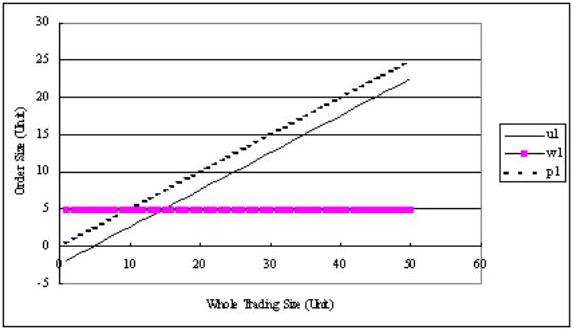
\includegraphics[width=10cm,height=6cm]{fg_l1n.png}
\end{center}
\caption[$R_1$ and $u_1^*$, $w_1^*$, and $p_1^*$ without constraints]
{{\bf $R_1$ ($x$-axis) and $u_1^*$, $w_1^*$, and $p_1^*$ ($y$-axis) without constraints.}
 \quad $u_1^*$, $w_1^*$, and $p_1^*$ are linear functions of $R_1$.}\label{fg_l1}
\end{figure}

\begin{figure}
\begin{center}
 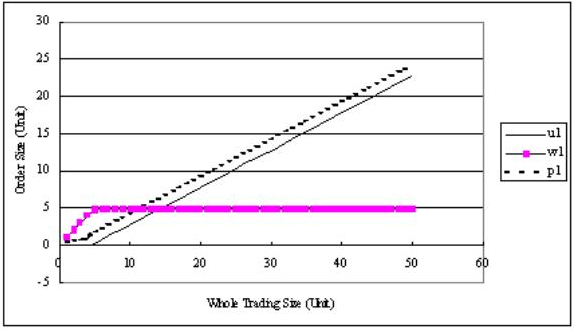
\includegraphics[width=10cm,height=6cm]{fg_l2n.png}
\end{center}
\caption[$R_1$ and $u_1^*$, $w_1^*$, and $p_1^*$ with non-negative constraint]
{{\bf $R_1$ ($x$-axis) and $u_1^*$, $w_1^*$, and $p_1^*$ ($y$-axis) with non-negative constraint.}
 \quad $u_1^*$, $w_1^*$, and $p_1^*$ are linear functions of $R_1$ for large $R_1$.}\label{fg_l2}
\end{figure}

%%%%%%%%%%%%%%%%%%%%%
\subsection{Multiple Period Case}\label{sec_l23}
The results in two period case can be extended to $T$ period case by Markov decision process since $C_1^*(R_1)$ is sum of square of $R_1$ and a constant.  Specifically, immediate application of two period case provides $T-1^{th}$ period strategy as
\[ %begin{equation}\label{eq_l19}
 \left\{
  \begin{array}{ll}
   \displaystyle p_{T-1}^* = -\frac{(ra_{T-1}-2a_T)a_{T-1}R_{T-1}}{2\{(1-r)a_{T-1}+a_T\}}, \\
   \displaystyle \frac{w_{T-1}^*}{2\sigma_{T-1}}= \frac{(1-r)a_{T-1}}{2\{(1-r)a_{T-1}+a_T\}}\frac{\phi(\frac{w_{T-1}^*}{2\sigma_{T-1}})}{\Phi(-\frac{w_{T-1}^*}{2\sigma_{T-1}})},\\
   \displaystyle u_{T-1}^*= \frac{p_{T-1}^*}{a_{T-1}}-\frac{w_{T-1}^*}{2},\\
  \end{array}
  \right.
\] %end{equation}
and the optimal cost is $\displaystyle C_{T-1}^*(R_{T-1})=\frac{\{4a_T-r^2a_{T-1}\}a_{T-1}}{4\{(1-r)a_{T-1}+a_T\}}R_{T-1}^2+constant.$  Since the optimal cost in the two period case is $a_2 R_2^2$, $i^{th}$ period strategy $(i=T-2,\cdots,1)$ is calculated similarly as
\[ %begin{equation}\label{eq_l20}
 \left\{
  \begin{array}{ll}
   \displaystyle p_i^* = -\frac{(ra_i-2A_i)a_iR_i}{2\{(1-r)a_i+A_i\}}, \\
   \displaystyle \frac{w_i^*}{2\sigma_i}= \frac{(1-r)a_i}{2\{(1-r)a_i+A_i\}}\frac{\phi(\frac{w_i^*}{2\sigma_i})}{\Phi(-\frac{w_i^*}{2\sigma_i})},\\
   \displaystyle u_i^*= \frac{p_i^*}{a_i}-\frac{w_i^*}{2}\\
  \end{array}
  \right.
\] %end{equation}
where $A_i\ (i=1,\cdots,T-1)$ is defined backward recursively as $\displaystyle
A_i=\frac{\{4A_{i+1}+r^2a_i\}a_i}{4\{(1-r)a_i+A_{i+1}\}}\ (i=T-2,\cdots,1)$ with
$\displaystyle A_{T-1}=\frac{\{4a_T+r^2a_{T-1}\}a_{T-1}}{4\{(1-r)a_{T-1}+a_T\}}$.

Figure \ref{fg_l3} shows a numerical example which illustrates changes of optimal market and limit order size over time.  In this numerical example, we assume that market order, all the realized $M_i$ turn out to be zero ($T=11, R_1=100, r=0, a_i=1, \sigma_i=10$ for $i=1,\cdots,11$).

\begin{figure}[htbp]
\begin{center}
 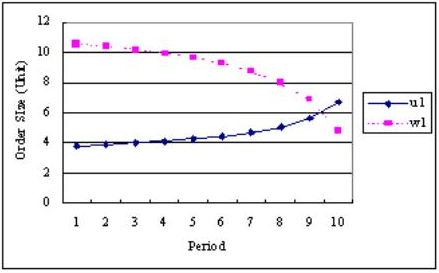
\includegraphics[width=10cm,height=6cm]{fg_l3n.png}
\end{center}
\caption[Time dependency of limit order and market order]
{{\bf Time dependency of limit order and market order} ($T=11$,
 $R_1=100$, $a_i=1$, $\sigma_i=10$ for $i=1, \cdots, 11$).
 \quad We assumed that market order, $M_i$, was revealed to be zero all the time.
 We can see that more limit orders are tried at the early stage of execution, and they are gradually replaced
with market orders.}\label{fg_l3}
\end{figure}

\begin{figure}[htbp]
\begin{center}
 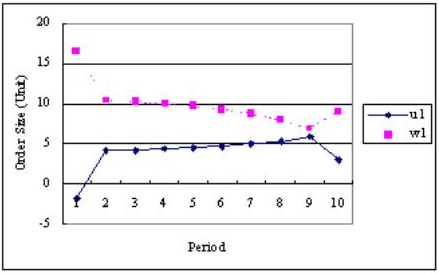
\includegraphics[width=10cm,height=6cm]{fg_l4n.png}
\end{center}
\caption[Time dependency of limit order and market order]
{{\bf Time dependency of limit order and market order} ($T=11$, $R_1=100$, $a_1=a_{11}=1.5$,
$\sigma_1=\sigma_{11}=15$, $a_i=1$, $\sigma_i=10$ for $i=2, \cdots, 10$).
 \quad We assumed that market order, $M_i$, was revealed to be zero all the time.
 Comparing to Figure \ref{fg_l3}, we can see that limit orders are avoided when $a_i$ and $\sigma_i$ are high
due to high expected cost, and market orders are preferred due to high option values.}\label{fg_l4}
\end{figure}

We can see that more limit orders are tried at the early stage of execution, and they are gradually replaced with market orders if limit orders are not executed.  Also, a case when $a_i$ and $\sigma_i$ depend on period is worth observing in order to analyze a whole day execution, since Jain and Joh (1988) find that $a_i$ and $\sigma_i$ are high at the opening and closing of a day.  Figure \ref{fg_l4} shows a numerical example in which $a_1=a_{11}=1.5$ and $\sigma_1=\sigma_{11}=15$, and all the other parameters are the same as in Figure \ref{fg_l3}.  Comparing to Figure \ref{fg_l3}, we can see that market orders are avoided when  $a_i$ and $\sigma_i$ are high due to high expected cost, and limit orders are preferred due to high option values.

Regarding statistical errors in estimating parameters, empirical studies such as Uno and Yamada (1993) and Jain and Joh (1988) report that the patterns of market impact coefficients, the price volatility, and the market trading volume are rather stable.

%%%%%%%%%%%%%
\section{Variations of Single Limit Order Model}\label{sec_l3}
In this section, we analyze several variations of the standard model in Section \ref{sec_l2}.  Although two period models are analyzed for clarity of comparison with the standard model, multiple period extension is possible in each case.

\subsection{Risk Averse Traders}
Since limit orders have uncertainty in execution, risk averse traders may prefer market orders.  When we measure risk by variance of total purchase amount, cost function can be defined as
\begin{eqnarray}\label{eq_l21}
  C_1(R_1) & = & \ex{ \sum_{j=2}^2 \delta_j \epsilon_j R_j + \sum_{i=1}^2 P_i \{(1-r) D_i +r R_i\}} \nonumber \\
      &   & +\lambda \var{ \sum_{j=2}^2 \delta_j \epsilon_j R_j + \sum_{i=1}^2 P_i \{(1-r) D_i +r R_i\}} \nonumber \\
      & = & \ex{ \sum_{i=1}^2 P_i \{(1-r) D_i +r R_i\}}+\lambda \var{\sum_{j=2}^2 \delta_j \epsilon_j R_j + \sum_{i=1}^2 P_i \{(1-r) D_i +r R_i\}}
\end{eqnarray}
where the definitions of $P_i$ and $D_i$ are the same as those in risk neutral case, $\lambda$ is a risk premium, and $V$ is the variance at the first period.

Although it is difficult to solve (\ref{eq_l21}), changes of fundamental cost tends to be much larger than the uncertainly of market impact in practice.  Therefore, we ignore uncertainty of market impact, which makes the solution a linear function as in the risk neutral case.  That is, cost function can be approximated by 
\begin{eqnarray*}\label{eq_l22}
  C_1(R_1) & \approx & \ex{\sum_{i=1}^2 P_i \{(1-r) D_i +r R_i\}}+\lambda \var{\delta_2 \epsilon_2 R_2} \nonumber \\
      & = & \ex{P_1 \{(1-r) D_1 +r R_1\}+a_2(R_1-D_1)^2}+\lambda \delta_2^2 \ex{ (R_1-D_1)^2}.
\end{eqnarray*}
Therefore, all we have to do is to replace $a_2$ of the solution in the risk neutral case with $(a_2+\lambda \delta_2^2)$.

Our optimal execution duration for risk averse traders is not very sensitive to trade size as in Almgren and Chriss (2001), which contradicts practical intuition.  This is because variance type risk measure is employed in order to implement dynamic programming.  As a result, it is recommended in practice to use both Konishi and Makimoto (2001) for execution scheduling problem and this analysis for order placing problem.

%%%%%%%%%%%%%%%%%%%%%%%%
\subsection{Visible Public Market Orders}
Up to this section, we assume that the trader knows just the expectation of the public limit orders and the distribution of the public market orders, but not concrete order sizes.  In this section however, we analyze the case when the trader monitors the public order book, and all the current period information is available.  Regarding the future periods, we continue to assume that the trader knows only the distribution and not the size of public market orders as in the previous cases.

As we have mentioned, not all traders can monitor all the public limit order books at TSE, only member security brokers are allowed to watch without time lag.  Also, even member security brokers have to choose which stocks to monitor among thousands of listed stocks.  This section estimates the value of monitoring public order books, comparing cost with that in Section \ref{sec_l2}.  

Let $b_1(p)$ and $s_1(p)$ denote volume of public buy and sell limit orders at price $p$ in the first period, respectively, and $M_i$ denote volume of excess public market order at the $i^{th}$ period.  Without loss of generality, we can assume that 
\[ %begin{equation}\label{eq_l23}
  \left\{
  \begin{array}{ll}
   b_1(p)=0, & \quad \mbox{if} \quad p>0, \\
   s_1(p)=0, & \quad \mbox{if} \quad p<0
  \end{array}
  \right.
\] %end{equation}
because buy limit order is synthesized by buy market order and sell limit order, and sell limit order is synthesized by sell market order and buy limit order.

Market orders, buy limit orders at higher price than execution price, and sell limit orders at lower price than execution price are executed, and the trader do not distinguish market and limit orders since not only market orders but also limit orders are surely executed.  Therefore, let $V_1$ denote the sum of the trader's market order and buy limit orders at higher prices than execution price.  Also, in order to complete the execution, we assume that all the remaining orders are placed as market order in the second period.  In this case, market impact $P_1$ is determined so as to balance total buy orders and sell orders.  Among them, since the trader's execution volume is $V_1$, expected purchase cost is $\ex{(P_1+Q_1)V_1}=P_1V_1$.  Also, execution volume of public buy and sell orders is $\displaystyle \int_{P_1}^{\infty} b_1(p) dp$ and $\displaystyle \int_{-\infty}^{P_1} s_1(p) dp$, respectively.  Therefore,
\[ %begin{equation}\label{eq_l24}
  V_1+M_1+\int_{P_1}^{\infty} b_1(p) dp-\int_{-\infty}^{P_1} s_1(p) dp=0.
\] %end{equation}

Regarding the second period, we assume that limit order exists at any prices for the constant amount $1/a_i$, and that the ratio of permanent market impact is $r$ as in the previous cases.  Consequently, there are sell limit orders of $1/a_i$ above price $Q_2+rP_1$ and buy limit orders of $1/a_i$ below price $Q_2+rP_1$ in the second period.  In this case, our problem can be formulated as follows:
\begin{equation}\label{eq_l25}
  \mbox{(P)} \ \ \left|
  \begin{array}{ll}
    \mbox{minimize} & \quad C_1(R_1)= P_1 \{(1-r) V_1 +r R_1\}+a_2(R_1-V_1)^2 \\
    \mbox{s.t.} & \displaystyle \quad V_1+M_1+\int_{P_1}^{\infty} b_1(p) dp-\int_{-\infty}^{P_1} s_1(p) dp=0.
  \end{array}
  \right.
\end{equation}
We can easily derive the optimal $V_1^*$ at least numerically once $Q_1$, $R_1$, $a_2$, $b_1(p)$, $s_1(p)$, and $M_1$ are given.


In the rest of this section, we analyze a linear market impact case in order to compare the results with those in Section \ref{sec_l2}:
\begin{eqnarray*}
  b_1(p) & = & \left\{
  \begin{array}{ll}
   0, & \quad \mbox{if} \quad p>0, \\
   \frac{1}{a_1}, & \quad \mbox{if} \quad p<0,
  \end{array}
  \right. \label{eq_l26}\\
  s_1(p) & = & \left\{
  \begin{array}{ll}
   \frac{1}{a_1}, & \quad \mbox{if} \quad p>0, \\
   0, & \quad \mbox{if} \quad p<0.
  \end{array}
  \right. \label{eq_l27}
\end{eqnarray*}
Since the constraint in (\ref{eq_l25}) is
\[ %begin{equation}\label{eq_l28}
  V_1+M_1=\frac{P_1}{a_1},
\] %end{equation}
our objective function is
\begin{eqnarray}\label{eq_l29}
  C_1(R_1) & = & P_1 \{(1-r) V_1 +r R_1\}+a_2(R_1-V_1)^2 \nonumber \\
      & = & \{(1-r)a_1+a_2\}V_1^2+[\{(1-r)M_1+rR_1\}a_1-2Ra_2]V_1+(rM_1a_1+2Ra_2).
\end{eqnarray}
$V_1$ which minimizes (\ref{eq_l29}) satisfies
\[ %begin{equation}\label{eq_l30}
  \pdif{C_1}{V_1}=2\{(1-r)a_1+a_2\}V_1+\{(1-r)M_1+rR_1\}a_1-2Ra_2=0.
\] %end{equation}
Therefore, the optimal order size $V_1^*$ is
\[ %begin{equation}\label{eq_l31}
  V_1^*=\frac{-\{(1-r)M_1+rR_1\}a_1+2R_1a_2}{2\{(1-r)a_1+a_2\}},
\] %end{equation}
and the optimal expected cost $C_1^*(R_1)$ is
\[ %begin{equation}\label{eq_l32}
  C_1^*(R_1) = \frac{-(1-r)^2a_1^2 M_1^2+2\{r(1-r)a_1+2a_2\}R_1 a_1 M_1+(4a_2-r^2a_1)a_1R_1^2}{4\{(1-r)a_1+a_2\}}.
\] %end{equation}
If we collect large samples in order to compare the optimal expected cost with the result in Section \ref{sec_l2}, $M_i$ follows normal distribution $N(0,\sigma_i)$.  Therefore, the average of $C_1^*(R_1)$ becomes
\[ %begin{equation}\label{eq_l33}
  \ol{C_1^*(R_1)} = \frac{(4a_2-r^2a_1)a_1R_1^2-(1-r)^2\sigma_1^2a_1^2}{4\{(1-r)a_1+a_2\}}.
\] %end{equation}
Difference between $\ol{C_1^*(R_1)}$ and the minimal cost in Section \ref{sec_l2} is
\[ %begin{equation}\label{eq_l34}
  \frac{-(1-r)^2\sigma_1^2a_1^2}{4\{(1-r)a_1+a_2\}} + \frac{\{(1-r)a_1+2a_2\}(1-r)a_1\sigma_1^2\phi^2(\frac{w_1}{2\sigma_1})}{2\{(1-r)a_1+a_2\}\Phi(\frac{w_1}{2\sigma_1})} - a_2\sigma_1^2\{2\Phi(\frac{w_1}{2\sigma_1})-1\},
\] %end{equation}
which corresponds to economical value of monitoring the public order book, which is significant when $a_1$ and $\sigma_1$ are large.  Since the trader is assumed to be risk neutral, economical value of monitoring seems independent of $R_1$.  However in practice, traders closely monitor stocks of large trades because risk averse traders try to avoid uncertainty of market impact, and because execution of larger trades takes a longer time, which makes the economical value of monitoring large.

As we have mentioned, at TSE, only member security brokers can monitor the public order book without time lag, but not general traders.  Therefore, the economical value of monitoring is a component of the membership value.  Also, even brokers have to pay some ``cost" of infrastructure and labors to monitor the public order book, and therefore, choose stocks to monitor among thousands of listed stocks.  Our formula evaluates the value of monitoring in order to justify costs of monitoring and provides criteria for selecting stocks to monitor.


%%%%%%%%%%%%%%%%%%%%%%%%%%%%%%
\section{Multiple Limit Order Model}\label{sec_l4}
Result of the standard model in Section \ref{sec_l2} can be extended to a case with $N$ limit orders.  However, since calculation is extremely complicated, it is difficult to derive explicit solution.  Therefore, in this section, we just explain some characteristics of the optimal execution strategy derived numerically.  We study two period case for simplicity.

Let $p_{ij}\ (i=1,\cdots,N, \ j=1,\cdots,T)$ and $w_{ij}\ (i=1,\cdots,N, \ j=1,\cdots,T)$ denote
$i^{th}$ base limit order prices at the $j^{th}$ period and size of corresponding limit order sizes
where $p_{ij}>p_{kj}$ for $i<k$.  Also, let $u_j$ denote market order size, and define $v_{0j} \define u_j$ and $\displaystyle v_{ij} \define v_{0j}+\sum_{k=1}^i w_{kj}.$  Then, similar calculation leads to the expected cost at the first period $C_1$ as
\begin{eqnarray}
  C_1 & = &  \{(1-r)a_1+a_2\}v_{01}^2+(ra_1-2a_2)R_1v_{01}+a_2R_1^2+Q_1R_1 \nonumber \\
      &   &  -\sum_{i=1}^N [\{(1-r)a_1+a_2\}(v_{i-1,1}+\frac{p_{i1}}{a_1})+(ra_1-2a_2)R_1] \nonumber \\
      &   & \quad \quad \{(v_{i-1,1}-\frac{p_{i1}}{a_1})\Phi(-\frac{1}{\sigma_1}(v_{i-1,1}-\frac{p_{i1}}{a_1}))-\sigma_1\phi(-\frac{1}{\sigma_1}(v_{i-1,1}-\frac{p_{i1}}{a_1}))\} \nonumber \\
      &   &  +\sum_{i=1}^N [\{(1-r)a_1+a_2\}(v_{i1}+\frac{p_{i1}}{a_1})+(ra_1-2a_2)R_1] \nonumber \\
      &   & \quad \quad \{(v_{i1}-\frac{p_{i1}}{a_1})\Phi(-\frac{1}{\sigma_1}(v_{i1}-\frac{p_{i1}}{a_1}))-\sigma_1\phi(-\frac{1}{\sigma_1}(v_{i1}-\frac{p_{i1}}{a_1}))\} \nonumber \\
      &   &  +a_2\sigma_1^2\sum_{i=1}^N \{\Phi(-\frac{1}{\sigma_1}(v_{i-1,1}-\frac{p_{i1}}{a_1}))-\Phi(-\frac{1}{\sigma_1}(v_{i1}-\frac{p_{i1}}{a_1}))\}. \label{eq_l35}
\end{eqnarray}
Also, the first order conditions of optimality is given as
\begin{eqnarray}
  \pdif{C_1}{v_{01}} & = &  2\{(1-r)a_1+a_2\}v_{01}+(ra_1-2a_2)R_1 - [2\{(1-r)a_1+a_2\}v_{01}+(ra_1-2a_2)R_1]
  \nonumber \\
  & & \times \Phi(-\frac{1}{\sigma_1}(v_{01}-\frac{p_{11}}{a_1}))
        +(1-r)a_1\sigma_1 \phi(-\frac{1}{\sigma_1}(v_{01}-\frac{p_{11}}{a_1})), \label{eq_l36} \\
  \pdif{C_1}{v_{k1}} & = & - [2\{(1-r)a_1+a_2\}v_{k1}+(ra_1-2a_2)R_1]\Phi(-\frac{1}{\sigma_1}(v_{k1}-\frac{p_{k+1,1}}{a_1})) \nonumber \\
  & & +(1-r)a_1\sigma_1 \phi(-\frac{1}{\sigma_1}(v_{k1}-\frac{p_{k+1,1}}{a_1})) + [2\{(1-r)a_1+a_2\}v_{k1}+(ra_1-2a_2)R_1] \nonumber \\
  & & \times \Phi(-\frac{1}{\sigma_1}(v_{k1}-\frac{p_{k1}}{a_1}))-(1-r)a_1\sigma_1 \phi(-\frac{1}{\sigma_1}(v_{k1}-\frac{p_{k1}}{a_1})), \label{eq_l37} \\
  \pdif{C_1}{v_{N1}} & = & [2\{(1-r)a_1+a_2\}v_{N1}+(ra_1-2a_2)R_1]\Phi(-\frac{1}{\sigma_1}(v_{N1}-\frac{p_{N1}}{a_1})) \nonumber \\
  & & -(1-r)a_1\sigma_1 \phi(-\frac{1}{\sigma_1}(v_{N1}-\frac{p_{N1}}{a_1})), \label{eq_l38} \\
  a_1\pdif{C_1}{p_{k1}} & = & + [2\{(1-r)a_1+a_2\}\frac{p_{k1}}{a_1}+(ra_1-2a_2)R_1]\Phi(-\frac{1}{\sigma_1}(v_{k-1,1}-\frac{p_{k1}}{a_1})) \nonumber \\
                     &   & +\{(1-r)a_1+2a_2\}\sigma_1 \phi(-\frac{1}{\sigma_1}(v_{k-1,1}-\frac{p_{k1}}{a_1}))
                           - [2\{(1-r)a_1+a_2\}\frac{p_{k1}}{a_1}+(ra_1-2a_2)R_1] \nonumber \\
     & & \times \Phi(-\frac{1}{\sigma_1}(v_{k1}-\frac{p_{k1}}{a_1}))-\{(1-r)a_1+2a_2\}\sigma_1 \phi(-\frac{1}{\sigma_1}(v_{k1}-\frac{p_{k1}}{a_1})). \label{eq_l39}
\end{eqnarray}

Figure \ref{fg_l5} compares the optimal costs derived numerically from (\ref{eq_l36}) to (\ref{eq_l39}) for various numbers of limit orders when $a_1=a_2=1$, $\sigma_1=10$, $r=0$, and $R_1=50$.  Although the optimal cost is a decreasing function of the number of limit orders, cost reduction decreases as the number of limit orders increases.  This result supports the effectiveness of the single limit order model.

Figure \ref{fg_l6} shows the corresponding optimal base limit order prices and their sizes.  We can see that the limit order size is symmetrical.  Although sizes increase as limit order prices depart from the center of symmetry, this is because limit orders are dense around the center.  The density of limit orders is unimodal, similar to the single limit order model.

\begin{figure}[htbp]
\begin{center}
 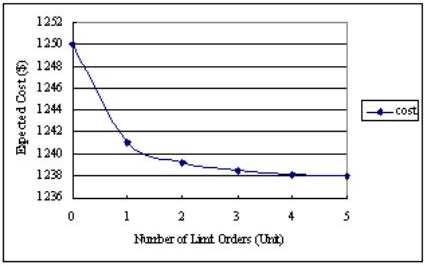
\includegraphics[width=10cm,height=6cm]{fg_l5n.png}
\end{center}
\caption[Number of limit orders and the expected cost]
{{\bf Number of limit orders ($x$-axis) and the expected cost ($y$-axis).}
 \quad This graph compares the optimal costs for various numbers of limit orders.
 Although the optimal cost is a decreasing function of the number of limit orders, cost reduction decreases as
the number of limit orders increases.
 This result supports the effect of the single limit order model.}\label{fg_l5}
\end{figure}

\begin{figure}[htbp]
\begin{center}
 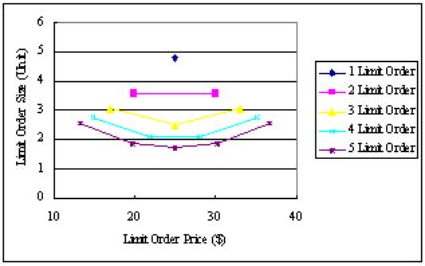
\includegraphics[width=10cm,height=6cm]{fg_l6n.png}
\end{center}
\caption[Optimal base limit order prices and their sizes]
{{\bf Optimal base limit order prices ($x$-axis) and their sizes ($y$-axis).}
 \quad We can see that the limit order size is indeed symmetrical.
 Although sizes increase as limit orders depart from the center of symmetry, this is because limit orders are
dense arround the center.
 The density of limit orders is unimodal, similar to single limit order model.}\label{fg_l6}
\end{figure}


Numerical solution suggests the following conjecture about the optimal solution although the proof of the optimality has not yet been completed. 
\begin{conjecture}\label{con_l1}
\begin{equation} \label{eq_l40}
 v_{i1}^*+v_{N-i,1}^* = \frac{p_{i+1,1}^*}{a_1} + \frac{p_{N-i,1}^*}{a_1} = -\frac{(ra_1-2a_2)R_1}{2{(1-r)a_1+a_2}}, \quad \mbox{for even } N,
\end{equation}
and
\begin{equation} \label{eq_l41}
 v_{i+1,1}^*+v_{N-i,1}^* = \frac{p_{i1}^*}{a_1} + \frac{p_{N-i,1}^*}{a_1} = -\frac{(ra_1-2a_2)R_1}{2{(1-r)a_1+a_2}}, \quad \mbox{for odd } N.
\end{equation}
\end{conjecture}

Conjecture \ref{con_l1} can be explained as follows.  First of all, because (\ref{eq_l35}) does not change even if we switch $\displaystyle v_{i1}-\frac{p_{i+1,1}}{a_1}$ and $\displaystyle -\left(v_{N-i,1}-\frac{p_{N-i,1}}{a_1}\right)$,
\[ %begin{equation} \label{eq_l101}
  v_{i1}^*-\frac{p_{i+1,1}^*}{a_1}=-\left(v_{N-i,1}^*-\frac{p_{N-i,1}^*}{a_1}\right).  
\] %end{equation}
If $N$ is even, because $\displaystyle v_{a\frac{N}{2}}^*-\frac{p_{\frac{N}{2}+1}^*}{a_1}=-(v_{a\frac{N}{2}}^*-\frac{p_{\frac{N}{2}}^*}{a_1})$ and $\displaystyle \pdif{C_1}{v_{a\frac{N}{2}}}=0$,
\[ %begin{equation} \label{eq_l102}
  v_{a\frac{N}{2}}^*=-\frac{(ra_1-2a_2)R_1}{2\{(1-r)a_1+a_2\}}.
\] %end{equation}
Also, because $\displaystyle v_{a\frac{N}{2}}^*-\frac{p_{\frac{N}{2}+1}^*}{a_1}=-(v_{a\frac{N}{2}}^*-\frac{p_{\frac{N}{2}}^*}{a_1})$,
\[ %begin{equation} \label{eq_l103}
  p_{\frac{N}{2}}^*+p_{\frac{N}{2}+1}^*=-\frac{(ra_1-2a_2)a_1R_1}{2\{(1-r)a_1+a_2\}}.
\] %end{equation}
Further, because $\displaystyle v_{a\frac{N}{2}-1}^*-\frac{p_{\frac{N}{2}}^*}{a_1}=-(v_{a\frac{N}{2}+1}^*-\frac{p_{\frac{N}{2}+1}^*}{a_1})$,
\[ %begin{equation} \label{eq_l104}
v_{a\frac{N}{2}-1}^*+v_{a\frac{N}{2}+1}^*=-\frac{(ra_1-2a_2)R_1}{2\{(1-r)a_1+a_2\}}.
\] %end{equation}
Similarly, because $\displaystyle v_{a\frac{N}{2}+i}^*-\frac{p_{\frac{N}{2}+i+1}^*}{a_1}=-(v_{a\frac{N}{2}-i}^*-\frac{p_{\frac{N}{2}-i}^*}{a_1})$,
\[ %begin{equation} \label{eq_l105}
p_{\frac{N}{2}-i}^*+p_{\frac{N}{2}+i+1}^*=-\frac{(ra_1-2a_2)a_1R_1}{2\{(1-r)a_1+a_2\}}.
\] %end{equation}
Also, since $\displaystyle v_{a\frac{N}{2}-i-1}^*-\frac{p_{\frac{N}{2}-i}^*}{a_1}=-(v_{a\frac{N}{2}+i+1}^*-\frac{p_{\frac{N}{2}+i+1}^*}{a_1})$,
\[ %begin{equation} \label{eq_l106}
v_{a\frac{N}{2}-i-1}^*+v_{a\frac{N}{2}+i+1}^*=-\frac{(ra_1-2a_2)R_1}{2\{(1-r)a_1+a_2\}.}
\] %end{equation}
Similar argument holds for the case if $N$ is odd.

By (\ref{eq_l40}) and (\ref{eq_l41}), we can reason by analogy that $p_{i1}$ and $v_{i1}$ are linear functions of $R_1$, and therefore, $w_{i1}$ are constants just as in the single limit order model.


%%%%%%%%%%%%%%%%%
\section{Closing Remarks}\label{sec_l5}
This chapter analyses the optimal selection of market and limit orders in a series of single price batch auctions when the expectation of the limit order book is given.  We derive the analytical solution of a single limit order model for risk neutral traders, and then extend the result for risk averse traders.  Regarding the execution at each period, we find that the optimal limit order size is independent of the whole trade size so as to balance the non-linearity of execution volume and price.  In contrast, the limit order price and the market order size are linear functions in order to balance trading costs across trading periods.  Regarding the execution throughout the trading session, market orders replace limit orders as time passes, and necessity of completing execution grows.  Further, if trading volume and price volatility are larger at the opening and closing of the trading session as in the practical markets, more limit orders are tried at the opening and closing.

Although most traders know the public order book as expectations as in our model, member security brokers are allowed to monitor the public order book without time lags.  So, we evaluate the value of monitoring public order books and provide criteria for selecting stocks to monitor.

Although our results can be extended to multiple limit order models mathematical analysis is left for further research.  Besides, while this chapter analyzes batch auctions for simplicity, continuous auction is also of interest.  Also, although this chapter assumes randomness comes only from the number of market orders, the number of limit orders are also stochastic in practice.  Further, we can extend our research to risk averse traders who uses VWAP as a reference price.  Besides, while this chapter performs partial equilibrium type analysis in which public orders are given exogenously, general equilibrium analysis which studies how each trader's strategy interferes is left for further research.

%%%%%%%%%%%%%%%%%%%%%
\section{Appendix}\label{sec_lappendix}

\subsection{Proof of Proposition \ref{prop_l1}}
In two period case,
\begin{eqnarray*} \label{eq_l42}
  C_1(R_1) & = & \ex{ \pi_1(\psi_1) \{(1-r) \kappa_1(\psi_1) + r R_1 \}+ a_2(R_1-\kappa_1(\psi_1,M_1)^2} \nonumber \\
      & = &  \int_{-(\u1)}^{\infty}\{a_1(m_1+u_1)\{(1-r)u_1+rR_1\}+a_2(R_1-u_1)^2\}f_1(m_1)dm_1 \nonumber \\
      &   &  +\int_{-(\v1)}^{-(\u1)}\{p_1\{(1-r)(-m_1+\frac{p_1}{a_1})+rR_1\}+a_2(R_1+m_1-\frac{p_1}{a_1})^2\}f_1(m_1)dm_1 \nonumber \\
      &   &  +\int_{-\infty}^{-(\v1)}\{a_1(m_1+v_1)\{(1-r)v_1+rR_1\}+a_2(R_1-v_1)^2\}f_1(m_1)dm_1 \nonumber \\
      & = &  \int_{-(\u1)}^{\infty}[a_1\{rR_1+(1-r)u_1\}m_1+(a_1+a_2-ra_1)u_1^2-(2a_2-ra_1)R_1u_1]f_1(m_1)dm_1 \nonumber \\
      &   &  +\int_{-(\v1)}^{-(\u1)} a_2m_1^2+\{2a_2R_1+((r-1)a_1-2a_2)\frac{p_1}{a_1}\}m_1 \nonumber \\
      &   & +\{(1-r)a_1+a_2\}(\frac{p_1}{a_1})^2+(ra_1-2a_2)R_1\frac{p_1}{a_1} ]f_1(m_1)dm_1 \nonumber \\
      &   &  +\int_{-\infty}^{-(\v1)}[a_1\{rR_1+(1-r)v_1\}m_1+(a_1+a_2-ra_1)v_1^2-(2a_2-ra_1)R_1v_1]f_1(m_1)dm_1 \nonumber \\
      &   & +a_2R_1^2.
\end{eqnarray*}
Using the following equations,
\begin{eqnarray*}
  \int_{-\infty}^{-a} x f_1(x) dx & = &  -\sigma_1^2 f_1(a),  \label{eq_l43}\\
  \int_{a}^{b} x^2 f_1(x)dx       & = &  \int_{a}^{b} \sigma_1^2 f_1(x)dx -[\sigma_1^2 x f_1(x)]_a^b,  \label{eq_l44}
\end{eqnarray*}
we obtain the following result,
\begin{eqnarray*} \label{eq_l45}
  C_1(R_1) & = &  \{(1-r)a_1+a_2\}v_{01}^2+(ra_1-2a_2)R_1v_{01}+a_2R_1^2 \nonumber \\
      &   &  - [\{(1-r)a_1+a_2\}(u_1+\frac{p_1}{a_1})+(ra_1-2a_2)R_1]\{(\u1)F_1(-(\u1))-\sigma_1^2f_1(-(\u1))\} \nonumber \\
      &   &  + [\{(1-r)a_1+a_2\}(v_1+\frac{p_1}{a_1})+(ra_1-2a_2)R_1]\{(\v1)F_1(-(\v1))-\sigma_1^2f_1(-(\v1))\} \nonumber \\
      &   &  +a_2\sigma_1^2 \{F_1(-(\u1))-F_1(-(\v1))\}
\end{eqnarray*}
where $F_1(x)= \int_{-\infty}^x f_1(y) dy.$
 The desired result now follows by noting
\[
 F_1(w) = \Phi(\frac{w}{\sigma_1}), \qquad \sigma_1^2 f_1(w) = \sigma_1 \phi(\frac{w}{\sigma_1})
\]
where $\displaystyle \phi(x)=\frac{1}{\sqrt{2\pi}}exp(-\frac{x^2}{2})$
and $\Phi(x)=\int_{-\infty}^x \phi(y) dy$.

%%%%%%%%%%%%%%
\subsection{Proof of Proposition \ref{prop_l2}}
Define $\displaystyle \overline{u}_1=\frac{\u1}{\sigma_1}$ and
$\displaystyle \overline{v}_1=\frac{\v1}{\sigma_1}$.
  Since
\begin{eqnarray}
 & & F_1(-(\u1))=\Phi(-\overline{u}_1), \label{eq_l46}\\
 & & F_1(-(\v1))=\Phi(-\overline{v}_1), \label{eq_l47}\\
 & & \displaystyle f_1(-(\u1))=\frac{1}{\sigma_1}\phi(-\overline{u}_1), \label{eq_l48}\\
 & & \displaystyle f_1(-(\v1))=\frac{1}{\sigma_1}\phi(-\overline{v}_1), \label{eq_l49}
\end{eqnarray}
$C_1(R_1)$ can be rewritten as,
\begin{eqnarray} \label{eq_l50}
  C_1(R_1) & = &  [\{(1-r)a_1+a_2\}(\frac{p_1}{a_1})^2+(ra_1-2a_2)R_1\frac{p_1}{a_1}+a_2\sigma_1^2] \nonumber \\
      &   &  +[\{(1-r)a_1+a_2\}(\sigma_1^2\overline{u}_1^2+2\sigma_1\frac{p_1}{a_1}\overline{u}_1)+(ra_1-2a_2)R_1\sigma_1\overline{u}_1-a_2\sigma_1^2]\Phi(\overline{u}_1) \nonumber \\
      &   &  +[\{(1-r)a_1+a_2\}(\sigma_1^2\overline{v}_1^2+2\sigma_1\frac{p_1}{a_1}\overline{v}_1)+(ra_1-2a_2)R_1\sigma_1\overline{v}_1-a_2\sigma_1^2]\Phi(-\overline{v}_1) \nonumber \\
      &   &  +[\{(1-r)a_1+a_2\}(\sigma_1^2\overline{u}_1+2\sigma_1\frac{p_1}{a_1})+(ra_1-2a_2)R_1\sigma_1]\phi(\overline{u}_1) \nonumber \\
      &   &  -[\{(1-r)a_1+a_2\}(\sigma_1^2\overline{v}_1+2\sigma_1\frac{p_1}{a_1})+(ra_1-2a_2)R_1\sigma_1]\phi(-\overline{v}_1) \nonumber \\
      &   &  +a_2R_1^2.
\end{eqnarray}
We then prove that the optimality and the uniqueness of the solution.  First, define 
\begin{eqnarray*}
  & & a = (1-r)a_1 + a_2, \qquad A = a_2, \qquad \sigma = \sigma_1, \\
  & & \beta = (ra_1 - 2a_2)R_1, \qquad \gamma = p_1/a_1, \qquad x = \overline{u}_1, \qquad y = \overline{v}_1,
\end{eqnarray*}
and
\[
  G(x) \define x \Phi(x) + \phi(x).
\]
Also, we represent function parameters by subscripts as $\Px = \Phi(x)$ and $\gx = G(x).$  According to (\ref{eq_l50}),
\begin{eqnarray}
  C_1(R_1)
   & = & a \gamma^2 + \beta \gamma + A \sigma^2 + [a (\sigma^2 x^2 + 2 \sigma x \gamma)
         + \beta \sigma x - A\sigma^2] \Px
         + [a (\sigma^2 y^2 + 2 \sigma y \gamma) + \beta \sigma y - A \sigma^2] \Pmy \nonumber \\
   &   & + [a (\sigma^2 x + 2\sigma \gamma) + \beta \sigma] \px
       - [a (\sigma^2 y + 2\sigma \gamma) + \beta \sigma] \py + A R_1^2  \nonumber \\
   & = & A \sigma^2 + AR_1^2 + a \gamma^2 + 2 a \sigma \left( x \Px + \px
         + y \Pmy - \py + \frac{\beta}{2a\sigma}  \right) \gamma \nonumber \\
   &   & + \sigma \left[ \left(
         a \sigma x^2 + \beta x - A \sigma \right) \Px + (a \sigma x + \beta) \px +
         \left( a \sigma y^2 + \beta y -A \sigma \right) \Pmy - (a \sigma y + \beta) \py
         \right] \nonumber \\
   & = & A\sigma^2 + AR_1^2 + a \gamma^2 + 2 a \sigma \left( \gx - \gmy
         + \frac{\beta}{2a\sigma} \right) \gamma \nonumber \\
   &   & + \sigma \left[ (a\sigma x + \beta) \gx - (a\sigma y + \beta) \gmy
         - A \sigma \{ \Px + \Pmy \} \right] \nonumber \\
   & = & A\sigma^2 + AR_1^2 + a \left[ \gamma + \sigma \left( \gx - \gmy
         + \frac{\beta}{2a\sigma} \right) \right]^2 \nonumber \\
   &   & + a \sigma^2 \left[ x \gx - y \gmy + \frac{\beta}{a\sigma} (\gx - \gmy) - \frac{A}{a} (\Px + \Pmy)
         \right] - a \sigma^2 \left( \gx - \gmy + \frac{\beta}{2a\sigma} \right)^2 \nonumber \\
   & = & A\sigma^2 + AR_1^2  - \frac{\beta^2}{4a} + a \left[ \gamma
         + \sigma \left( \gx - \gmy + \frac{\beta}{2a\sigma} \right) \right]^2 \nonumber \\
   &   & + a \sigma^2 \left[ x \gx - y \gmy - \frac{A}{a} ( \Px + \Pmy )
         - \left( \gx - \gmy \right)^2 \right]. \label{eq_l51}
\end{eqnarray}
Define the quotient of the last term of (\ref{eq_l51}) by $a \sigma^2$ as
\[ %begin{equation}\label{eq_l52}
  H(x,y) \define x \gx - y \gmy - \frac{A}{a} ( \Px + \Pmy )
        - \left( \gx - \gmy \right)^2.
\] %end{equation}
We minimize $C_1$ on $\calS = \{ (x,y)\ : \ -\infty < x <\infty, y \geq x \}$.

\begin{lemma}\label{lem_l1}
  \quad The minimum of $H$ exists on $\calS$.
\end{lemma}

\begin{proof}
Since $H(x,y)=H(-y,-x)$, $H(x,y)$ is symmetrical about $y=-x$.  Therefore, we have only to analyze on
 $\calS' = \{ (x,y)\ : -\infty < x < \infty, y \geq |x| \}.$  According to Abramowitz and Stegun (1972) p.932,
\[ %begin{equation}\label{eq_l53}
  \frac{\px}{x} \left( 1 - \frac{1}{x^2} + \frac{3}{x^4} - \frac{15}{x^6} \right) <
  \Pmx < \frac{\px}{x} \left( 1 - \frac{1}{x^2} + \frac{3}{x^4} + \frac{15}{x^6} \right), \qquad
  x > 0,
\] %end{equation}
and therefore,
\begin{eqnarray*}
  & & x + \px \left( \frac{1}{x^2} - \frac{3}{x^4} - \frac{15}{x^6} \right) < \gx
      < x + \px \left(\frac{1}{x^2} - \frac{3}{x^4} + \frac{15}{x^6} \right), \qquad x > 0, \label{eq_l54} \\
  & & \px \left( \frac{1}{x^2} - \frac{3}{x^4} - \frac{15}{x^6} \right) < \gmx
      < \px \left(\frac{1}{x^2} - \frac{3}{x^4} + \frac{15}{x^6} \right), \qquad x > 0. \label{eq_l55}
\end{eqnarray*}
Consequently, limits along the point $\calS'$ where $(sy,y)\ (-1 \leq s \leq 1)$ is given by
\[
 \lim_{y \rightarrow + \infty} H(sy,y) = \left\{
 \begin{array}{ll}
   -A/a, \quad & s > 0, \\
   -A/2a+\p0^2, & s = 0, \\
   0, & s < 0.
 \end{array}
 \right.
\]
Therefore, $H(x,y)$ is a function bounded from the bottom.  Further, since $H(0,0)=-A/a \leq \lim_{y \rightarrow +\infty} H(sy,y)$, $H(x,y)$ takes the minimum at a finite $(x,y)$.
\end{proof}

Since $\gamma$ can take any value, the minimization of $C$ by $(x, y, \gamma)$ is equivalent to the minimization of $H$ by $(x, y)$ with $\gamma = - \sigma ( \gx - \gmy + \beta/2a\sigma ).$  From the first order condition of the optimality,
\begin{eqnarray}
  \pdif{H}{x}
   & = & \gx + x \Px - \frac{A}{a} \px - 2 ( \gx - \gmy ) \Px = 0, \label{eq_l56} \\
  \pdif{H}{y}
   & = & - \gmy + y \Pmy + \frac{A}{a} \py - 2 ( \gx - \gmy ) \Pmy = 0 \label{eq_l57}
\end{eqnarray}
are necessary conditions.  By canceling $A/a$ from (\ref{eq_l56}) and (\ref{eq_l57}),
\begin{eqnarray*}
  \lefteqn{\py \left[ \gx + x \Px - 2 ( \gx - \gmy ) \Px \right]
    + \px \left[ - \gmy + y \Pmy - 2 ( \gx - \gmy ) \Pmy \right]} \nonumber \\
  & & \hspace{1.0cm} = 2 \py \Px [ x - ( \gx - \gmy )] + 2 \px \Pmy [ y - ( \gx - \gmy )] \nonumber \\
  & & \hspace{1.0cm} = 2 [ \py \Px ( \gmy - \gmx ) + \px \Pmy ( \gy - \gx ) ] \nonumber \\
  & & \hspace{1.0cm} = 0. \label{eq_l58}
\end{eqnarray*}
Define
\[ %begin{equation}\label{eq_l59}
  I(x,y) \define \px \Pmy (\gy - \gx) + \Px \py (\gmy - \gmx),
\] %end{equation}
and we have the following lemma.
\begin{lemma}\label{lem_l6}
 \quad For any $x$, $I(x,x)=I(x,-x)=0$.  Further, for any $x$ and $y > |x|$, $I(x,y)>0$.
\end{lemma}

Lemma \ref{lem_l6} shows that the first order condition of the optimality is satisfied only by $y=x$ and $y=-x$.  If we substitute $y=x$ (\ref{eq_l56}), we have
\begin{eqnarray*}
 \left. \pdif{H}{x} \right|_{y=x}
  & = & \gx + x \Px - \frac{A}{a} \px - 2 ( \gx - \gmx ) \Px \\
  & = & \gx + x \Px - \frac{A}{a} \px - 2 x\Px \\
  & = & \px - \frac{A}{a} \px \\
  & = & 0,
\end{eqnarray*}
which contradicts $0<A/a<1$.  Next, if we substitute $y=-x$, we have
\begin{equation}\label{eq_l60}
  \left. \pdif{H}{x} \right|_{y=-x} = 2 x \Phi(x) + \left( 1 - \frac{A}{a} \right) \phi(x) = 0.
\end{equation}
Regarding the solution of (\ref{eq_l60}), we have the following lemma.
\begin{lemma}\label{lem_l2}
 \quad Define $M(x) \define (ax+b)\Phi(x)+c\phi(x)$ where $a>0$ and $a>c$.  Then, $M(x)=0$ has a unique solution with positive derivative.
\end{lemma}
\begin{proof}
Direct calculation shows that
\[ %begin{equation} \label{eq_l61}
  M'(x)=a\Phi(x)+b\phi(x)+(a-c)x\phi(x),
\] %end{equation}
and
\[ %begin{equation} \label{eq_l62}
  M''(x)=\phi(x)\{-(a-c)x^2-bx+(2a-c)\}.
\] %end{equation}
Therefore, $M''(x)=0$ has two real solutions across which $M''(x)$ turns from negative to positive once, and then negative again.  Together with $\displaystyle \lim_{x \to -\infty} M'(x) =0$ and $\displaystyle \lim_{x \to \infty} M'(x) = a>0$, $M'(x)$ has a unique solution $x^*$ and,
\begin{equation} \label{eq_l63}
 \left\{
  \begin{array}{ll}
   M'(x)<0, \quad x<x^*, \\
   M'(x)>0, \quad x>x^*.
  \end{array}
  \right.
\end{equation}
Further, together with $\displaystyle \lim_{x \to -\infty} M(x) =0$ and $\displaystyle \lim_{x \to \infty} M(x) = \infty$, $M(x)=0$ has a unique solution where $M'(x)>0$.
\end{proof}

By Lemma \ref{lem_l2}, $x$ that satisfies (\ref{eq_l60}) is uniquely determined.  Consequently, $x=x^*$ is determined as the unique solution of (\ref{eq_l60}), and then, $y^* = -x^*$ and $\gamma^* = -\beta/2a$.

\bigskip

\noindent {\bf Proof of Lemma \ref{lem_l6}} \quad
It is easy to show $I(x,x)=I(x,-x)=0$.  We consider the case of $y>|x|$.  We first calculate partial derivatives of $I$ by $y$.  
\begin{eqnarray*}
  I_1(x,y)
   & \define & \frac{\partial}{\partial y} I(x,y) \\
   & = & \Px (-y \py \gmy - \py \Pmy) + \px (-\py \gy + \Pmy \Py) + \Px \gmx y \py + \px \gx \py, \\
  I_2(x,y)
   & \define & \frac{\partial}{\partial y} I_1(x,y) \\
   & = & \py [ \Px \{ (y^2-1) \gmy + 2y \Pmy + \py \} + \px (y\gy + 1 - 3\Py) -(y^2-1)\Px\gmx - \px \gx y ], \\
  J_2(x,y)
   & \define & \Px \{ (y^2-1) \gmy + 2y \Pmy + \py \} + \px (y\gy + 1 - 3\Py) -(y^2-1)\Px\gmx - \px \gx y, \\
  J_3(x,y)
   & \define & \frac{\partial}{\partial y} J_2(x,y) \\
   & = & \Px \{ 2y \gmy - (y^2-3) \Pmy -3y\py \} + \px ( \gy +y \Py -3\py ) -2 \Px \gmx y - \px \gx, \\
  J_4(x,y)
   & \define & \frac{\partial}{\partial y} J_3(x,y) \\
   & = & 2 [ \Px \{ \gmy - 2y \Pmy + (2y^2-3) \py \} + \px (\Py + 2y \py) - \Px \gmx ], \\
  J_5(x,y)
   & \define & \frac{\partial}{\partial y} J_4(x,y) \\
   & = & 2 [ \Px \{ -3 \Pmy -(2y^3-9y) \py \} - \px (2y^2-3) \py ], \\
  J_6(x,y)
   & \define & \frac{\partial}{\partial y} J_5(x,y) \\
   & = & 2 \py \{ (2y^4-15y^2+12) \Px + (2y^3-7y) \px \}.
\end{eqnarray*}
Since 
\[
 I(x,y) \approx \px \Pmy \gy - \Px \gmx \py \approx \Pmx \gx \py
\]
for $y \rightarrow +\infty$, we obtain\footnote{For a function $f$, we define $f(\pm \infty)=\lim_{t \rightarrow \pm \infty} f(t)$.  Also, $a+0\ (a-0)$ represents conversion to $a$ from the above (from the below)}
\[
 I(x,+\infty) = 0+0.
\]
Together with $I(x,x) = I(x,-x) = 0$, if we prove the existence and the uniqueness of $y>|x|$ where $I_1(x,y)=0$ for any $x$, we can prove that $I(x,y)>0$ for $y>|x|$.

In order to see the sign change of $J_6$, we first analyze
\[
 K(y) \define \frac{2y^4-15y^2+12}{2y^3-7y} = y - \frac{8y^2-12}{2y^3-7y}.
\]
Then,
\begin{eqnarray*}
  \dif{K}{y}
    & = & 1 + \frac{16y^4 - 16y^2 +84}{(2y^3-7y)^2} \\
    & = & 1 + \frac{4 (2y^2 - 1)^2 +80}{(2y^3-7y)^2} \\
    & > & 0, \qquad\qquad (\forall x \neq 0, \pm \sqrt{7/2}).
\end{eqnarray*}
Therefore, $K(y)$ is monotone increasing for $y \neq 0, \pm \sqrt{7/2}$, and shifts according to the following table.
\[
\begin{array}{|c||c|c|c|c|c|c|c|c|c|c|c|c|c|c|} \hline
  y & -\infty & \cdots & \multicolumn{2}{c|}{{\displaystyle -\frac{\sqrt{15+\sqrt{129}}}{2}}} & \cdots
    & \multicolumn{2}{c|}{{\displaystyle -\sqrt{\frac{7}{2}}}} & \cdots
    & \multicolumn{2}{c|}{{\displaystyle -\frac{\sqrt{15-\sqrt{129}}}{2}}} & \cdots & \multicolumn{2}{c|}{0} \\ \hline
  2y^4-15y^2+12 & +\infty & + & \multicolumn{2}{c|}{0} & - & \multicolumn{2}{c|}{-} & - & \multicolumn{2}{c|}{0} & +
    & \multicolumn{2}{c|}{+} \\ \hline
  2y^3-7y & -\infty & - & \multicolumn{2}{c|}{-} & - & \multicolumn{2}{c|}{0} & + & \multicolumn{2}{c|}{+} & +
    & \multicolumn{2}{c|}{0} \\ \hline
  K(y) & -\infty & \nearrow & \multicolumn{2}{c|}{0} & \nearrow & +\infty & -\infty & \nearrow & \multicolumn{2}{c|}{0}
    & \nearrow & +\infty & -\infty \\ \hline
\end{array}
\]
\[
\begin{array}{|c||c|c|c|c|c|c|c|c|c|c|c|c|c|c} \hline
  y & \multicolumn{2}{c|}{0} & \cdots & \multicolumn{2}{c|}{{\displaystyle \frac{\sqrt{15-\sqrt{129}}}{2}}} & \cdots
    & \multicolumn{2}{c|}{{\displaystyle \sqrt{\frac{7}{2}}}} & \cdots
    & \multicolumn{2}{c|}{{\displaystyle \frac{\sqrt{15+\sqrt{129}}}{2}}} & \cdots & +\infty \\ \hline
  2y^4-15y^2+12 & \multicolumn{2}{c|}{+} & + & \multicolumn{2}{c|}{0} & - & \multicolumn{2}{c|}{-} & -
    & \multicolumn{2}{c|}{0} & + & +\infty \\ \hline
  2y^3-7y & \multicolumn{2}{c|}{0} & - & \multicolumn{2}{c|}{-} & - & \multicolumn{2}{c|}{0} & +
    & \multicolumn{2}{c|}{+} & + & +\infty \\ \hline
  K(y) & +\infty & -\infty & \nearrow & \multicolumn{2}{c|}{0} & \nearrow & +\infty & -\infty & \nearrow
    & \multicolumn{2}{c|}{0} & \nearrow & +\infty \\ \hline
\end{array}
\]
Since $J_6(x,y)=2 \py \Px (2y^3-7y) [K(y) + \px/\Px]$, $J_6(x,y)$ turns from ``positive, negative, positive, negative, and positive" for $y=-\infty \rightarrow +\infty$.  Henceforth, we represent this shifts as\footnote{Although we are interested only the area of $y>|x|$, we analyze the change of the sign for $y=-\infty \riinf$}

\begin{equation}\label{eq_l64}
 \sgn(J_6) = (+-+-+).
\end{equation}
Next, we analyze the sign change of $J_5$.
\begin{eqnarray}
  J_5(x,-\infty) & = & - 6 \Px \ \ < 0, \label{eq_l65} \\
  J_5(x,+\infty) & = & \lim_{y \rightarrow +\infty} -4 \Px y^3 \py = 0-0. \label{eq_l66}
\end{eqnarray}
By (\ref{eq_l64}), (\ref{eq_l65}), and (\ref{eq_l66}), three cases are possible for the sign change of $J_5$, $\sgn(J_5)=(-),\ (-+-),\ (-+-+-)$.  We next show that $\sgn(J_5)=(-+-+-)$ is not viable.  When $x$ is given, we define the smallest $y$ as $y_*$ among four $y$ that satisfy $J_6(x,y)=0$.  Then, $y_*<-\sqrt{15+\sqrt{129}}/2$.\footnote{Although $y_*$ depends on $x$, we do not write $x$ explicitly for the simplicity of the representation.  Besides, $y_*<-\sqrt{15+\sqrt{129}}/2$ holds for any $x$.}
Since $J_6(x,y_*)=0,$
\begin{eqnarray*}  
  J_5(x,y_*)
   & = & - 2 \Px (2y_*^2-3) \phi_{y_*} \left\{ \frac{3 \Phi_{-y_*} + (2y_*^3-9y_*)\phi_{y_*}}{(2y_*^2-3)\phi_{y_*}}
         + \frac{\px}{\Px} \right\} \\
   & = & - 2 \Px (2y_*^2-3) \phi_{y_*} \left\{ \frac{3\Phi_{-y_*} + (2y_*^3-9y_*)\phi_{y_*}}{(2y_*^2-3)\phi_{y_*}}
         - \frac{2y_*^4-15y_*^2+12}{2y_*^3-7y_*} \right\}.
\end{eqnarray*}

\begin{lemma}\label{lem_l3}
 \quad For any $x$, $J_5(x,y^*)<0.$
\end{lemma}

\begin{proof}
Since $2y_*^2-3>0$, it is sufficient to show $L(y^*)>0$ where
\[
  L(y) \define \frac{3\Phi_{-y} + (2y^3-9y)\phi_{y}}{(2y^2-3)\phi_{y}} - \frac{2y^4-15y^2+12}{2y^3-7y}.
\]
Since $y_* < -\sqrt{15+\sqrt{129}}/2<-2$, it is sufficient to show $L(y)>0$ for $y<-2$.
\[
 L(y) = \frac{1}{2y^2-3} \left( \frac{3\Pmy}{\py} + \frac{4y^4-6y^2+36}{2y^3-7y} \right)
      = \frac{1}{2y^2-3} \left( \frac{3\Pmy}{\py} + 2y + \frac{4}{y} + \frac{8}{2y^3-7y} \right).
\]
Since both $4/y$ and $8/(2y^3-7y)$ are decreasing for $y<-2$,
\[
 \frac{4}{y} + \frac{8}{2y^3-7y} > \frac{4}{-2} + \frac{8}{2 \cdot (-2)^3-7 \cdot (-2)} = -4.
\]
Consequently,
\[
 L(y) > \frac{1}{2y^2-3} \left( \frac{3 \Phi_{2}}{\sqrt{2\pi}} e^{y^2/2} + 2y -4 \right)
      > \frac{1}{2y^2-3} \left( 1.137 e^{y^2/2} + 2y -4 \right), \qquad y < -2.
\]
When we define
\[
 M(y) \define 1.136 e^{y^2/2} + 2y -4,
\]
we obtain
\[
 M(-2) > 0, \qquad\quad
 \dif{M}{y} = 1.136 y e^{y^2/2} + 2 < 0, \qquad \forall y<-2.
\]
Therefore, we have shown $M(y)>0$ for $y<-2$, i.e., $L(y)>0$.
\end{proof}

Since Lemma \ref{lem_l3} shows that the first relative minimum of $J_5$ is negative, $\sgn(J_5)=(-+-+-)$ never happens, and therefore, only $\sgn(J_5)=(-),\ (-+-)$ are possible cases.

Next, regarding the sign change of $J_4$,
\begin{eqnarray*}
 J_4(x,-\infty) & = & \lim_{y \rightarrow -\infty} - 6 \Px y = + \infty, \label{eq_l67} \\
 J_4(x,+\infty) & = & 2 \Pmx \gx \ \ > 0. \label{eq_l68}
\end{eqnarray*}
Together with $\sgn(J_5)=(-),\ (-+-)$, there are two possible cases, $\sgn(J_4)=(+),\ (+-+)$.

Next, regarding the sign change of $J_3$,
\begin{eqnarray*}
 J_3(x,-\infty) & = & \lim_{y \rightarrow -\infty} - 3 \Px y^2 = - \infty, \label{eq_l69} \\
 J_3(x,+\infty) & = & \lim_{y \rightarrow +\infty} 2 \Pmx \gx y = + \infty. \label{eq_l70}
\end{eqnarray*}
Together with $\sgn(J_4)=(+),\ (+-+)$, there are two possible cases, $\sgn(J_3)=(-+),\ (-+-+)$.

Next, regarding the sing change of $J_2$,
\begin{eqnarray*}
 J_2(x,-\infty) & = & \lim_{y \rightarrow -\infty} - \Px y^3 = + \infty, \label{eq_l71} \\
 J_2(x,+\infty) & = & \lim_{y \rightarrow +\infty} \Pmx \gx y^2 = + \infty. \label{eq_l72}
\end{eqnarray*}
Together with $\sgn(J_3)=(-+),\ (-+-+)$, there are two possible cases,
\begin{equation}\label{eq_l73}
 \sgn(J_2)=(+), \quad (+-+), \quad (+-+-+).
\end{equation}

Finally, regarding the sign change of $I_1$,
\begin{eqnarray}
 I_1(x,-\infty) & = & \lim_{y \rightarrow -\infty} \Px y^2 \py = 0 + 0, \label{eq_l74} \\
 I_1(x,x) & = & 0, \label{eq_l75} \\
 I_1(x,+\infty) & = & \lim_{y \rightarrow +\infty} - \Pmx \gx y \py = 0 - 0. \label{eq_l76}
\end{eqnarray}

\bigskip

\noindent (I) When $x \geq 0$
The following lemma holds for
\[
  J_2(x,x)=2 x \Px \Pmx + \px - 2\px \Px.
\]
\begin{lemma}\label{lem_l4}
\begin{equation}\label{eq_l77}
 J_2(x,x) \quad \left\{
 \begin{array}{ll}
 > 0, \quad & x>0, \\
 = 0, \quad & x=0, \\
 < 0, \quad & x<0.
 \end{array}
 \right.
\end{equation}
\end{lemma}
\begin{proof}
When we define
\[
 A(x) \define J_2(x,x) = 2x \Px \Pmx + \px - 2 \px \Px,
\]
\begin{eqnarray*}
 A_1(x) & \define & \dif{}{x}A(x) = 2 \Px \Pmx + 2x \px \Pmx - x \px - 2 \px^2, \\
 A_2(x) & \define & \dif{}{x}A_1(x) = \px ( 4 \Pmx - 2 \Px - 2 x^2 \Pmx+ 2 x \px -1 + x^2), \\
 B(x) & \define &  4 \Pmx - 2 \Px - 2 x^2 \Pmx+ 2 x \px -1 + x^2, \\
 B_1(x) & \define & \dif{}{x}B(x)= -2 \left( 2 \px + 2 x \Pmx - x \right)
             =      -4x \left( \frac{\px}{x} + \Pmx - \frac{1}{2} \right), \\
 C(x) & \define & \frac{\px}{x} + \Pmx - \frac{1}{2}, \\
 C_1(x) & \define & \dif{}{x}C(x) = - \px \left( 2 + \frac{1}{x^2} \right).
\end{eqnarray*}
Since $C_1(x)<0$ for any $x \neq 0$, and
\begin{eqnarray*}
  C(-\infty) & = & 1/2, \\
  C(0-0) & = & -\infty, \\
  C(0+0) & = & +\infty, \\
  C(+\infty) & = & -1/2,
\end{eqnarray*}
and toghether with $B_1(x) = -4x C(x),$
\begin{equation}\label{eq_l78}
 \sgn(B_1) = (+-+), \qquad x = -\infty \rightarrow +\infty.
\end{equation}
With (\ref{eq_l78}) and
\begin{eqnarray*}
  B(-\infty) & = & - \infty, \\
  B(0) & = & 0, \\
  B(+\infty) & = & + \infty, \\
  B_1(0) & = & -4 \p0 < 0,
\end{eqnarray*}
we obtain
\begin{equation}\label{eq_l79}
  \sgn(B) = \sgn(A_2) = (-+-+), \qquad x = -\infty \rightarrow +\infty.
\end{equation}
With (\ref{eq_l79}) and
\begin{eqnarray*}
  A_1(-\infty) & = & 0-0, \\
  A_1(0) & = & \frac{1}{2} - \frac{1}{\pi} > 0, \\
  A_1(+\infty) & = & 0-0,
\end{eqnarray*}
we obtain
\begin{equation}\label{eq_l80}
  \sgn(A_1) = (-+-).
\end{equation}
With (\ref{eq_l80}) and
\begin{eqnarray*}
  A(-\infty) & = & 0-0, \\
  A(0) & = & 0, \\
  A(+\infty) & = & 0+0,
\end{eqnarray*}
we finally obtain
\[ %begin{equation}\label{eq_l81}
  A(x) \ \ \left\{
  \begin{array}{ll}
   > 0, \quad & x>0, \\
   = 0, & x=0, \\
   < 0, & x<0.
  \end{array}
  \right.
\] %end{equation}
\end{proof}

By Lemma \ref{lem_l4}, when $x>0$, $I_1(x,y)$ crosses the $x$-axis from the negative to positive at $y=x$.  Also, when $I_1(x,y)$ moves from positive to positive at $y=x$.  In both cases, $I_1(x,y)=0$ has the unique solution on $y>|x|=x$ by equations from (\ref{eq_l73}) to (\ref{eq_l76}).\footnote{By this argument, $\sgn(J_2)=(+),\ (+-+)$ never happens actually.}

\bigskip

\noindent (II) When $x<0$
The following lemma holds for
\[
 I_1(x,-x) = \px \{ x^2 \Px + x \px + \Px (\Pmx - \Px) \}.
\]

\begin{lemma}\label{lem_l5}
 \quad For any $x \neq 0$, $I_1(x,-x)>0.$
\end{lemma}
\begin{proof}
\begin{eqnarray*}
  A(x) & \define & \frac{I_1(x,-x)}{\px} = x \gx + \Px - 2 \Px^2, \\ 
  A_1(x) & \define & \dif{}{x}A(x) = 2 (\gx - 2\px \Px), \\
  A_2(x) & \define & \dif{}{x}A_1(x) = 2(\Px + 2x \px \Px - 2\px^2), \\
  A_3(x) & \define & \dif{}{x}A_2(x) = 2\px (1+2\Px-2x^2 \Px + 6x \px), \\
  B(x) & \define & 1+2\Px-2x^2 \Px + 6x \px, \\
  B_1(x) & \define & \dif{}{x}B(x) = 4 ( 2 \px - x\Px - 2 x^2 \px ), \\
  B_2(x) & \define & \dif{}{x}B_1(x) = 4 [(2x^3 - 7x) \px - \Px], \\
  B_3(x) & \define & \dif{}{x}B_2(x) = - 4 \px (2x^4-13x^2+8)
\end{eqnarray*}
\noindent 1) Regarding $B_3$

Since $\sgn(2x^4-13x^2+8)=(+-+-+)$, we obtain $\sgn(B_3)=(-+-+-)$.  Also, $B_3(x)=0$ when
\[
 x = \pm \frac{\sqrt{13 \pm \sqrt{105}}}{2}.
\]

\smallskip

\noindent 2) Regarding $B_2$

Two relative maximums are
\begin{eqnarray*}
 B_2 \left( -\frac{\sqrt{13-\sqrt{105}}}{2} \right) & \approx & 1.1159, \\
 B_2 \left( \frac{\sqrt{13+\sqrt{105}}}{2} \right) & \approx & -0.7488.
\end{eqnarray*}
Also, since $B_2(-\infty) = 0-0$, and $B_2 (+\infty) = -4+0$, we obtain $\sgn(B_2)=(-+-).$

\smallskip

\noindent 3) Regarding $B_1$

Since $B_1(-\infty) = 0-0$, $B_1(0) = 8 \p0$, and $B_1(+\infty) = - \infty$, we obtain $\sgn(B_1)=(-+-)$.

\smallskip

\noindent 4) Regarding $B$

Since $B(-\infty) = 1-0$, $B(0) = 2$, and $B(+\infty) = -\infty$, we obtain either $\sgn(B)=\sgn(A_3)=(+-)$, or $(+-+-)$.

\smallskip

\noindent 5) Regarding $A_2$

Since $A_2(-\infty) = 0+0$, and $A_2(+\infty) = 2+0$, we obtain either $\sgn(A_2)=(+)$, or $(+-+)$.

\smallskip

\noindent 6) Regarding $A_1$

Since $A_1(-\infty) = 0+0$, $A_1(0) = 0$, $A_1(+\infty) = +\infty$, and $A_2(0) > 0$, we obtain $\sgn(A_1)=(+-+).$ \footnote{Therefore, $\sgn(A_2)=(+)$ never happens.}

\smallskip

\noindent 7) Regarding $A$

Since $A(-\infty) = 0+0$, $A(0) = 0$, $A(+\infty) = +\infty$, and $A_1(0) = 0$, we obtain $\sgn(A)=(+)$.
\end{proof}

By Lemma \ref{lem_l5} and (\ref{eq_l75}), there exists an area where
$I_1(x,y)$ increases on $y \in (x, -x)$.  By equations from
(\ref{eq_l73}) to (\ref{eq_l76}), $I_1(x,y)=0$ has a unique solution
over $y>|x|=-x$.\footnote{By this argument, $\sgn(J_2)=(+),\ (+-+)$
never happens actually. }

